The LASCAR (LASer CAlibration Rod) card (Fig. \ref{fig:laslascar}) is a masterpiece of the LASERII electronics scheme. This innovative board aims at controlling the \las~system thanks to the following components:
\begin{itemize}

\item digitization through a charge analog-to-digital converter (QDC)

\item charge injection (LILAS) to monitor the stability of the electronics (photodiode preamplifiers)

\item time-to-digital converter (TDC) to estimate the time response of the \las~as a function of its intensity

\item TTCRX : chip used to retrieve LHC signals

\item HOLA card : sends data fragments 

\item LASER interface : to drive the \las~(power, trigger)

\end{itemize}

\begin{figure}[htbp]

\centering
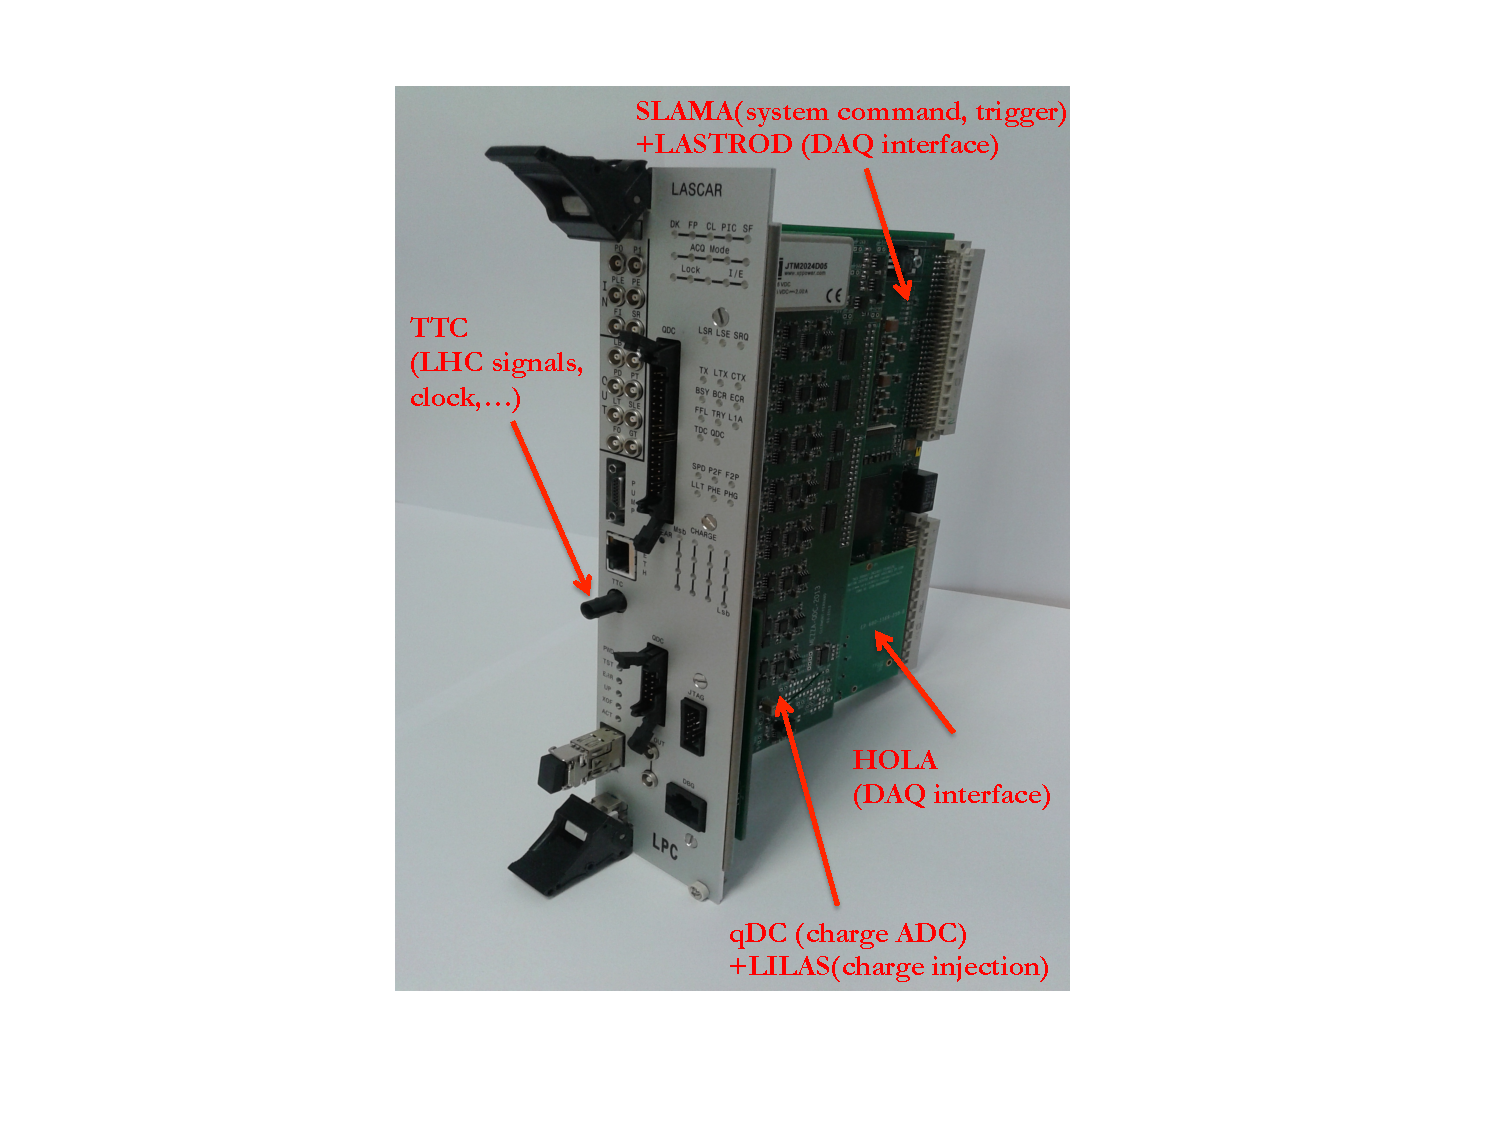
\includegraphics[height=10cm]{figures/Lascar_photo.pdf}
\caption{View of the LASCAR card}\label{fig:laslascar}
\end{figure}

The LASCAR card is housed in a VME crate and its adress is in the format A32/D32. The heart is composed of an Field Programmable Gate Array (FPGA) Cyclone V manufactured by ALTERA \cite{altera-cyclone}.

The following inputs-outputs (Fig. \ref{fig:laslascarlinks}) are available :
\begin{itemize}
\item 16 analogic channels (differential mode) for the QDC
\item 4 digital entries (NIM format)
\item 2 analogic entries for the photomultipliers
\item 8 digital outputs (NIM format)
\item 1 analogic-digital interface with the \las
\item one fiber (entry) to get information from the TTC
\item one fiber (input-output) for acquisition
\item one ethernet link for the DCS
\item one interface with the VME bus
\item one JTAG interface to configure the FPGA

\end{itemize}

\begin{figure}[htbp]

\centering
\includegraphics[height=15cm,width=15cm]{figures/Lascarlinks.pdf}
\caption{Scheme of the LASCAR card}\label{fig:laslascarlinks}
\end{figure}


\paragraph{QDC}

The QDC of the LASCAR module (Fig. \ref{fig:laslascarqdc}) comprises 32 channels, each with a 14-bit, high speed, low power, successive approximation ADC that operates from a single 2.5 V power supply and features throughput rates of up to 4.2 MSPS. Each channel contains two ADCs, each preceded by a low noise, wide bandwidth track-and-hold circuit that can handle input frequencies in excess of 110 MHz. This part is preceded by two charge amplifier with different slopes (x1 and x4). The analog signal at the entrance of the QDC is integrated during 500 ns (adjustable through a VME register) and the maximum charge that may be integrated is of about 2000 pC. Analog signals that are to be converted arise from the eleven photodiodes, the two PMTs, and from the charge injection system (3 channels, one internal to the QDC, and 2 from the photodiode box). 
 
\begin{figure}[htbp]

\centering
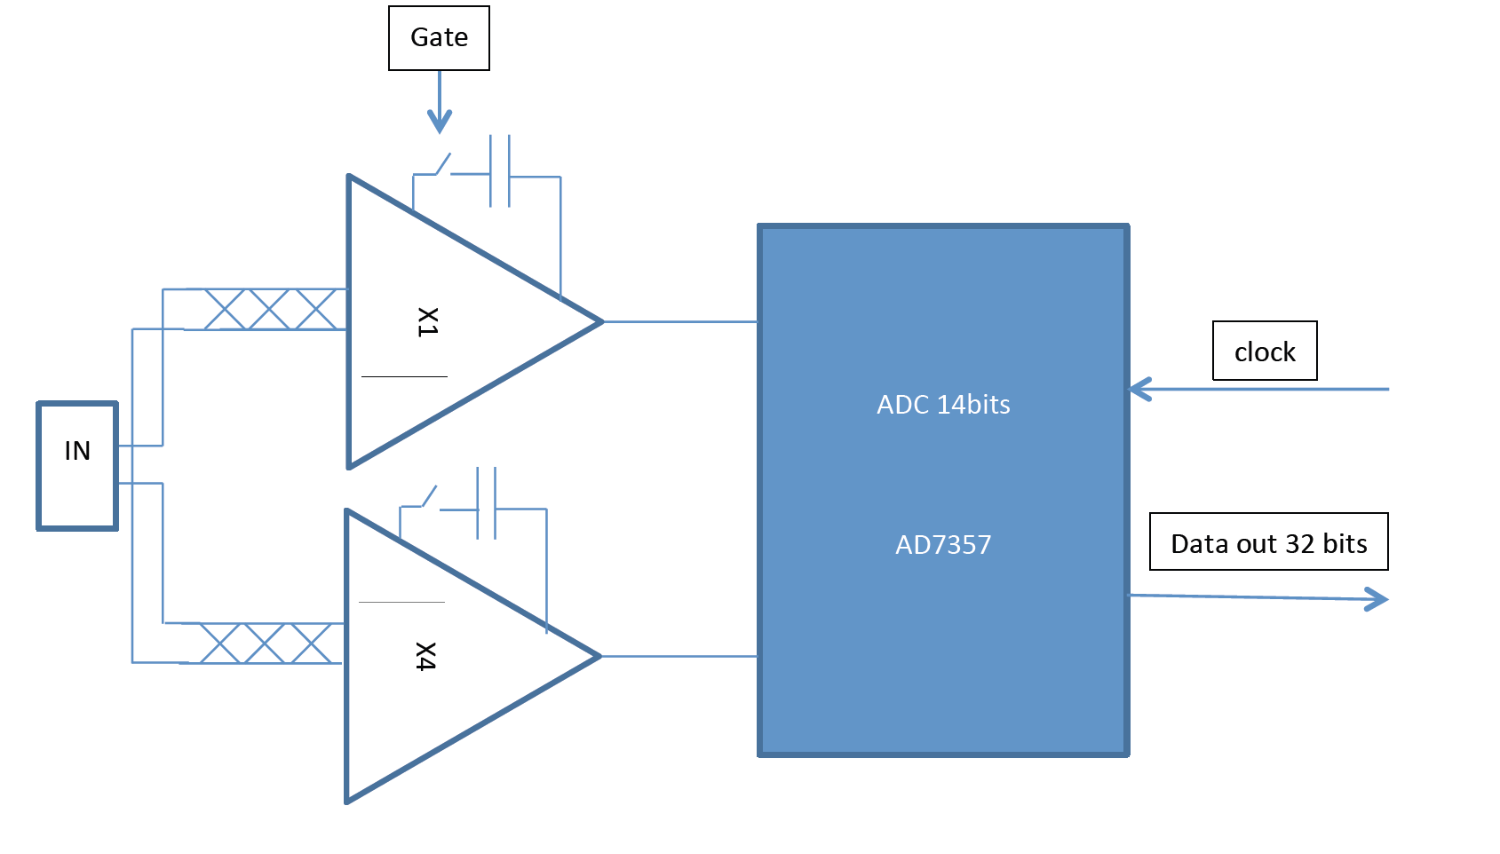
\includegraphics[height=5cm]{figures/qdc.pdf}
\caption{Scheme of the LASCAR QDC}\label{fig:laslascarqdc}
\end{figure}

\paragraph{LILAS}
The LILAS part of LASCAR (Fig. \ref{fig:laslascarlilas}) aims at injecting a known charge in each photodiode preamplifier so as to survey the linearity and the stability with time. The charge is injected in the system through three ways : a direct link to one of the QDC channels (since the QDC and LILAS are located on the same printed board), and two lemo cables plugged in the photodiode box and in Phocal.  

\begin{figure}[htbp]

\centering
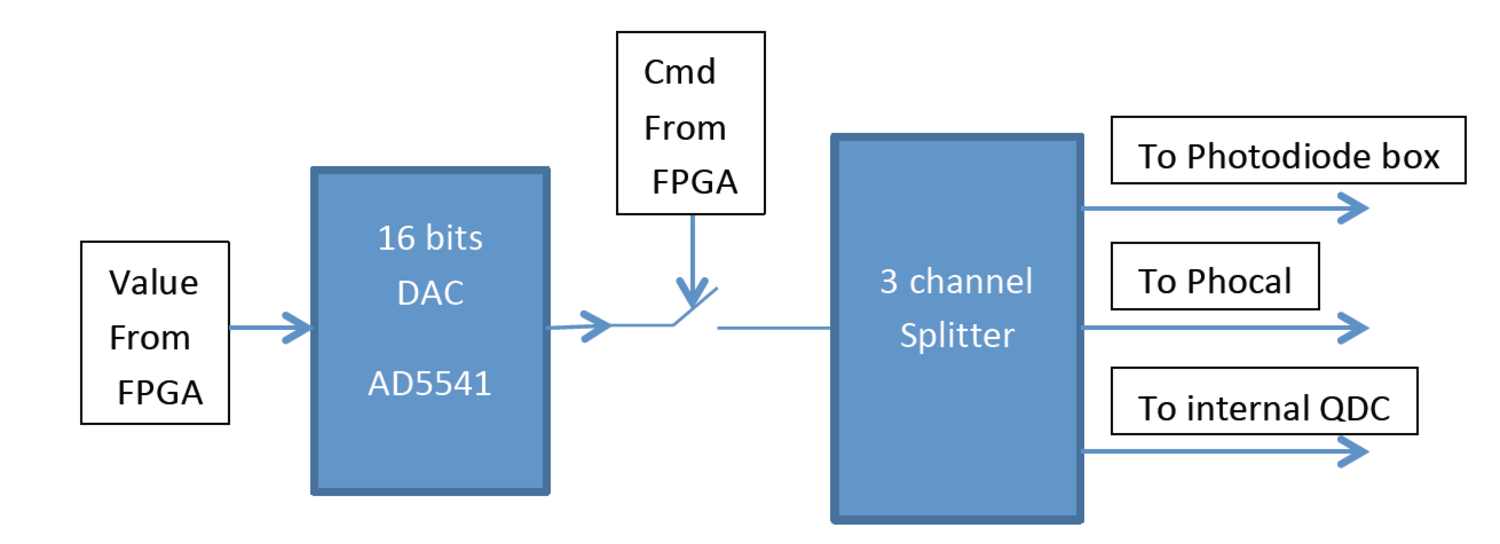
\includegraphics[height=5cm]{figures/lilas.pdf}
\caption{Scheme of the LASCAR LILAS}\label{fig:laslascarlilas}
\end{figure}

\paragraph{TDC}
The LASCAR TDC (Fig. \ref{fig:laslascartdc}) is a TDC-GP1, an integrated device manufactured by ACAM. It contains two measuring channels with a typical resolution of 280 ps. This TDC aims at measuring the \las~time response as a function of its power. The time response as a function of the intensity has been measured for the \las~we are using (Fig. \ref{fig:lasresponse}). Values around 420 ps are observed for lower intensities and a decrease to 320 ps is seen for higher intensities. LASCAR is equipped with a delay system so as to to send the \las~light in an "empty" bunch-crossing in a coherent way during the physics runs of the LHC.

\begin{figure}[htbp]

\centering
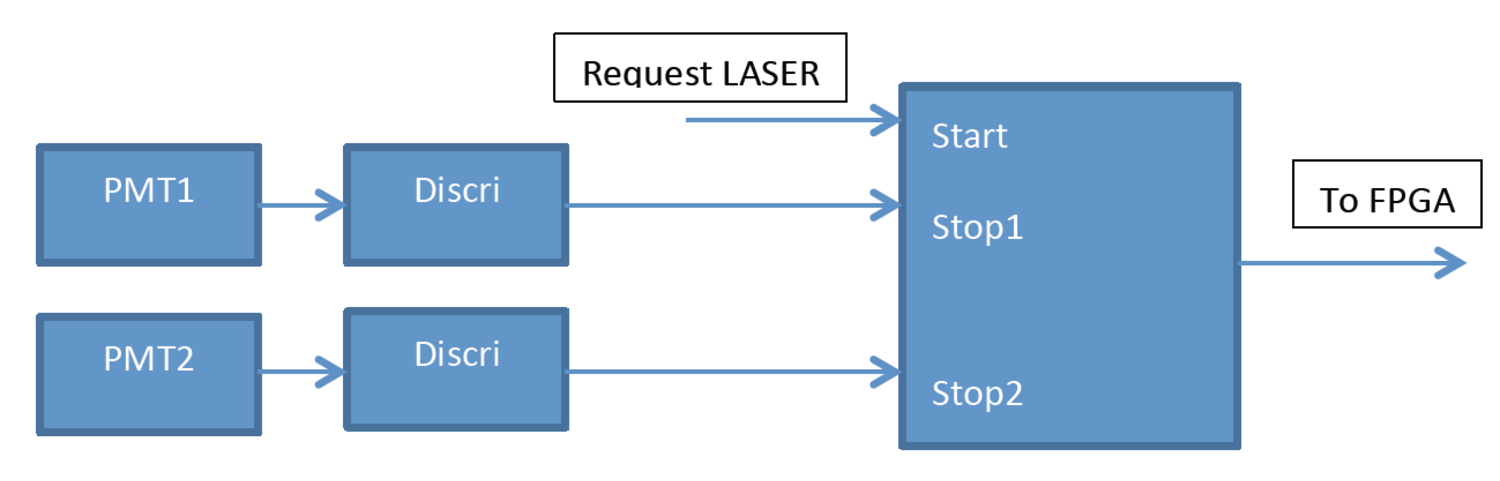
\includegraphics[height=5cm]{figures/tdc.pdf}
\caption{Scheme of the LASCAR TDC}\label{fig:laslascartdc}
\end{figure}

\begin{figure}[htbp]
\centering
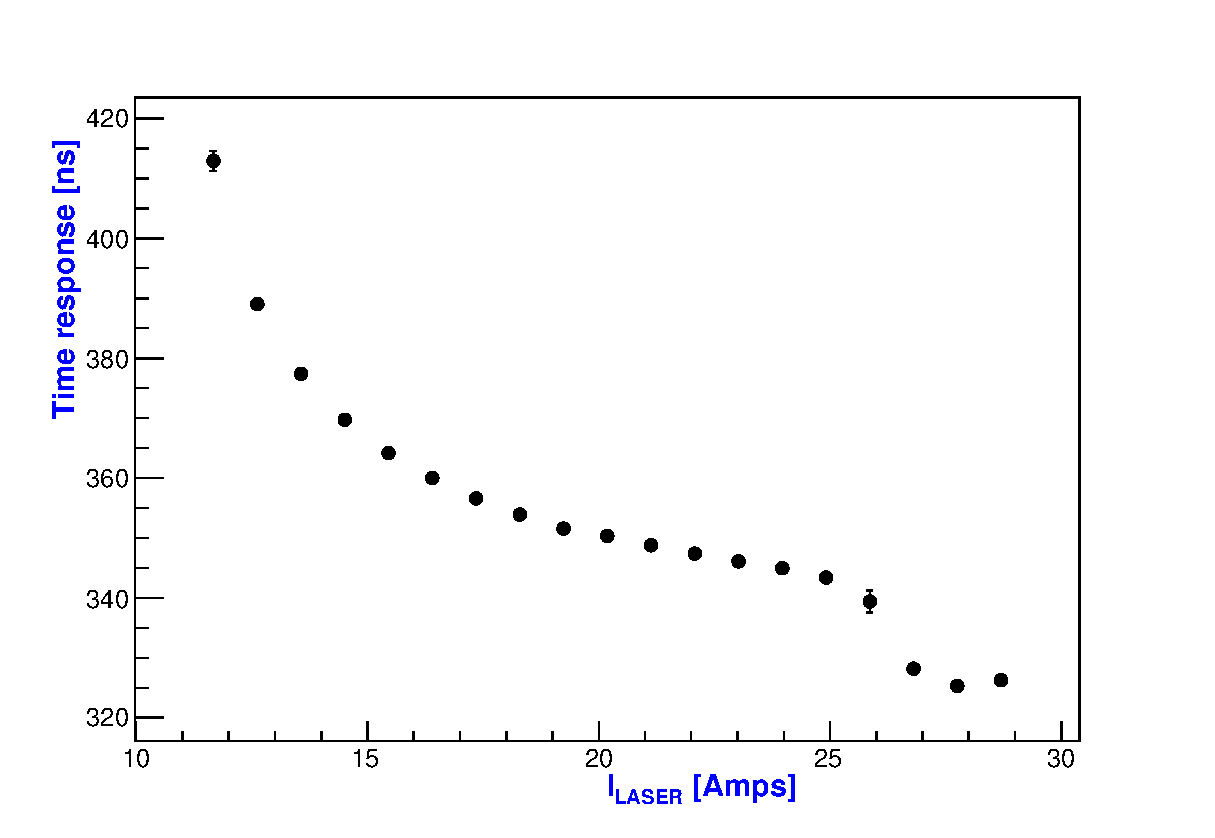
\includegraphics[height=10cm]{figures/laser_timing_new.eps}
\caption{\las~time response as a function of the intensity.}\label{fig:lasresponse}
\end{figure}

\paragraph{TTCRX}

The TTCRX is an integrated circuit developped at CERN that retrieves the following LHC signals :
\begin{itemize}
\item Bunch Crossing (BC)
\item Bunch Crossing Reset (BCR)
\item Event Counter Reset (ECR)
\item Level one Accept (L1A)
\item Level one Identity (L1AID)
\end{itemize}

The FPGA will process these data prior to  a transmission to the TDAQ.

\paragraph{HOLA}


\begin{figure}[htbp]

\centering
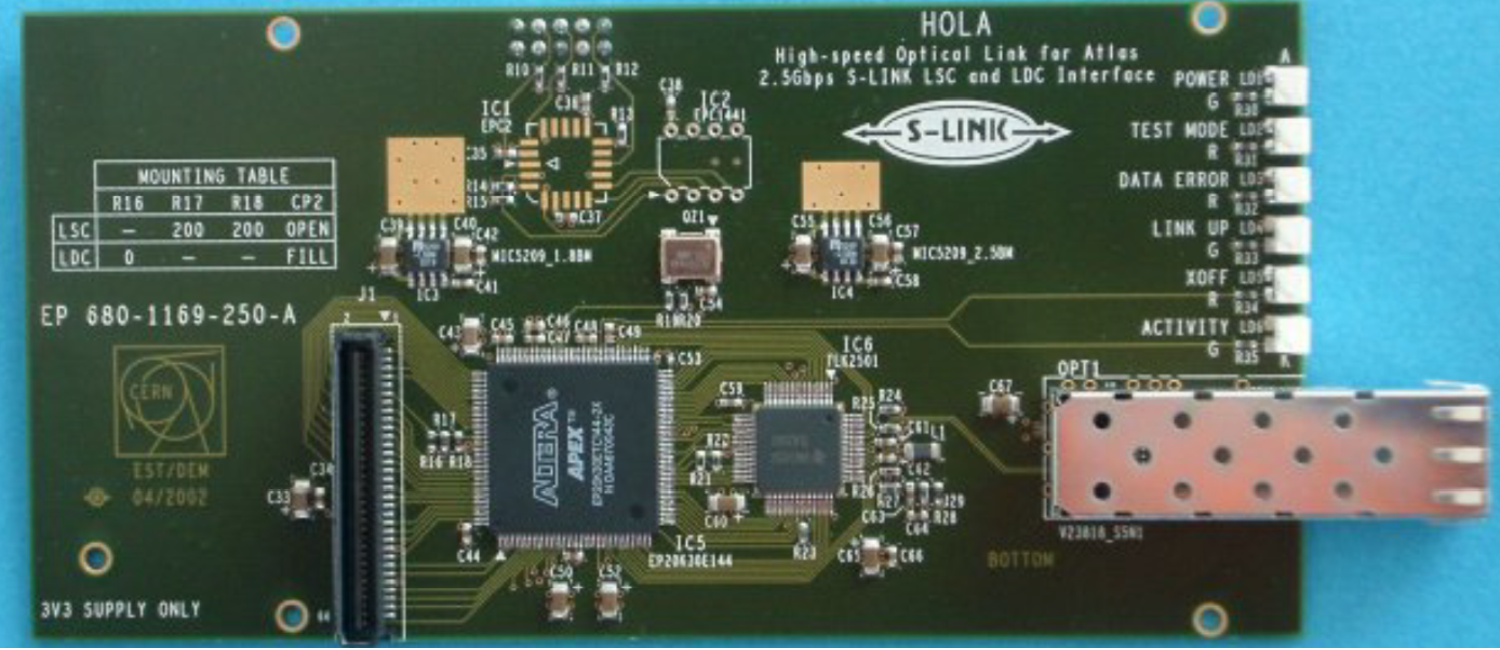
\includegraphics[height=5cm]{figures/hola.pdf}
\caption{View of the LASCAR HOLA}\label{fig:laslascarhola}
\end{figure}

\paragraph{LASER interface}

\begin{figure}[htbp]

\centering
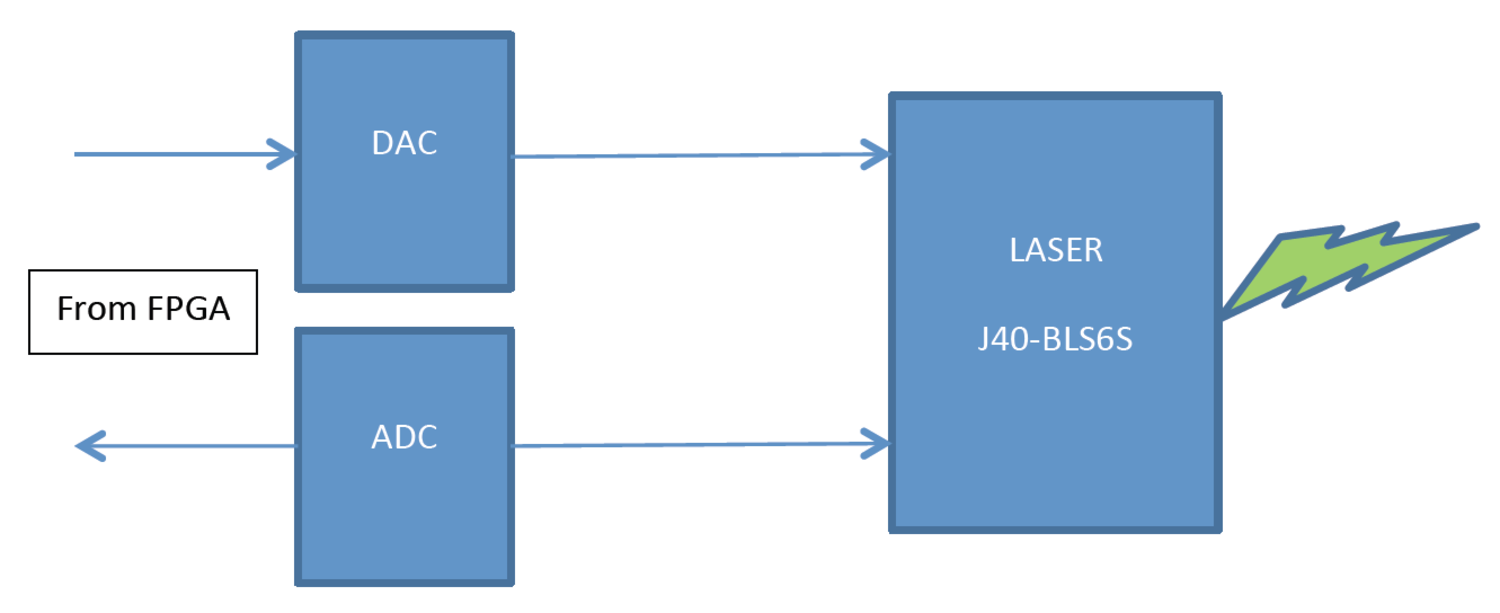
\includegraphics[height=5cm]{figures/laser_interface.pdf}
\caption{Scheme of the LASCAR LASER interface}\label{fig:laslascarlaserint}
\end{figure}

\paragraph{Acquisition modes}